\section{KHOẢNG CÁCH}
\subsection{KIẾN THỨC CẦN NHỚ}
\subsubsection{Khoảng cách từ một điểm đến một đường thẳng}
\immini{
	Cho điểm $O$ và một đường thẳng $a$. Trong $\left(O,a \right)$ gọi $H$ là hình chiếu vuông góc của $O$ trên $a$. Khi đó 
	\begin{gachsoc}
		\begin{itemize}
			\item [$\bullet$] Độ dài đoạn $OH$ được gọi là khoảng cách từ điểm $O$ đến $a$.
			\item [$\bullet$] Kí hiệu $\mathrm{d}\left(O,a \right)=OH.$
		\end{itemize} 
	\end{gachsoc}
}{ 
	\begin{tikzpicture}[scale=.7, font=\footnotesize, line join=round, line cap=round,>=stealth]
		\tkzInit[xmin=-1,xmax=7,ymin=-1,ymax=3] 
		\tkzClip
		\tkzDefPoints{0/0/A, 5/0/B,  2/2/D}
		\tkzDefPointsBy[translation= from A to B](D){C}
		\tkzDrawSegments(A,B B,C C,D D,A)
		\tkzDefPoints{1.5/.3/E, 6/1.5/F, 2/1.5/O}
		\tkzDrawSegments(E,F)
		\tkzLabelSegment(E,F){$a$}
		\coordinate (H) at ($(E)!0.3!(F)$);
		\tkzLabelPoints[right,below](H)
		\tkzLabelPoints[right](O)
		\tkzDrawPoints[fill=black](O,H)
		\tkzMarkRightAngles(O,H,F)
		\tkzDrawSegments(O,H)
		\tkzMarkAngles[size=0.7](B,A,D)
		\tkzLabelAngle[pos=.4](D,A,B){$\alpha$}
\end{tikzpicture} }
\subsubsection{Khoảng cách từ một điểm tới một mặt phẳng}
\immini{
	Cho mặt phẳng $\left(\alpha \right)$ và một điểm $O$, gọi $H$ là hình chiếu vuông góc của điểm $O$ trên mặt phẳng $\left(\alpha \right)$. Khi đó 
	\begin{gachsoc}
		\begin{itemize}
			\item [$\bullet$] Độ dài đoạn $OH$ được gọi là khoảng cách từ điểm $O$ đến mặt phẳng $\left(\alpha \right)$. Kí hiệu $\mathrm{d}\left(O,\left(\alpha \right)\right)=OH$.
			\item [$\bullet$] Ta luôn có $OH\le OM,\ \forall M\in \left(\alpha \right)$.
		\end{itemize}
	\end{gachsoc} 
	
}{
	\begin{tikzpicture}[scale=.7, font=\footnotesize, line join=round, line cap=round,>=stealth]
		\tkzDefPoints{0/0/A, 5/0/B,  2/2/D, 4.5/3/O, 4.5/1/H, 2.5/1/M,3.5/2/E, 4.5/2/F}
		\tkzDefPointsBy[translation= from A to B](D){C}
		\tkzDrawSegments(A,B B,C C,F E,D D,A O,H H,M M,O)
		\tkzDrawSegments[dashed](E,F)
		\tkzDrawPoints[fill=black](O,M,H)
		\tkzLabelPoints[above](O)
		\tkzLabelPoints[left]( M)
		\tkzLabelPoints[right](H)
		\tkzMarkRightAngles(O,H,M)
		\tkzMarkAngles[size=0.7](B,A,D)
		\tkzLabelAngle[pos=.4](D,A,B){$\alpha$}
	\end{tikzpicture}
}
\subsubsection{Khoảng cách từ một đường thẳng tới một mặt phẳng song song}
\immini{
	Cho đường thẳng $a$ song song với mặt phẳng $\left(\alpha \right)$. Khoảng cách giữa đường thẳng $a$ và mặt phẳng $\left(\alpha\right ) $ là khoảng cách từ một điểm bất kì của $a$ đến  mặt phẳng $\left(\alpha \right)$.
	\begin{gachsoc}
		\begin{itemize}
			\item [$\bullet$] Kí hiệu $\mathrm{d}(a,(\alpha)).$
			\item [$\bullet$] Nhận xét: $\mathrm{d}(a,(\alpha))=\mathrm{d}(A,(\alpha))=\mathrm{d}(B,(\alpha))$, với  $A,B \in a$.
		\end{itemize}
	\end{gachsoc}
}{
	\begin{tikzpicture}[scale=.6, font=\footnotesize, line join=round, line cap=round,>=stealth]
		\tkzInit[xmin=-1,xmax=7,ymin=-1,ymax=5] 
		\tkzClip
		\tkzDefPoints{0/0/A', 5/0/B',  2/2/D', 4.5/3/O, 4.5/1/H, 2.5/1/M,3.5/2/E, 4.5/2/F, 1.5/4/A1,  5.5/4/B1}
		\tkzDefPointsBy[translation= from A' to B'](D'){C'}
		\tkzDrawSegments(A',B'  B',C' C',D'  D',A'  A1,B1)
		\tkzLabelSegment[above](A1,B1){$a$}
		\tkzDefPointBy[projection= onto A1--B1](M) \tkzGetPoint{A}
		\tkzLabelPoints[above](A)
		\tkzDefPointBy[projection= onto A1--B1](H) \tkzGetPoint{B}
		\tkzLabelPoints[above](B)
		\tkzDrawSegments(A,M H,B)
		\tkzDrawPoints[fill=black](A,B,M,H)
		\tkzLabelPoints[below](H, M)
		\tkzMarkAngles[size=0.9](B',A',D')
		\tkzLabelAngle[pos=.5](D',A',B'){$\alpha$}
	\end{tikzpicture}	
}

\subsubsection{Khoảng cách giữa hai mặt phẳng song song}
\immini{
	Cho hai mặt phẳng $\left(\alpha \right)$ và $\left(\beta \right)$ song song với nhau, khoảng cách từ một điểm bất kì trên mặt phẳng này đến mặt phẳng kia được gọi là khoảng cách giữa hai mặt phẳng $\left(\alpha \right)$ và $\left(\beta \right)$.
	\begin{gachsoc}
		\begin{itemize}
			\item [$\bullet$] Kí hiệu $\mathrm{d}\left(\left(\alpha \right),\left(\beta \right)\right)$.
			\item [$\bullet$] Nhận xét $\mathrm{d}\left(\left(\alpha \right),\left(\beta \right)\right)=\mathrm{d}\left(M,\left(\beta \right)\right)$, với $M \in (\alpha)$.
		\end{itemize}
	\end{gachsoc}	
}{
	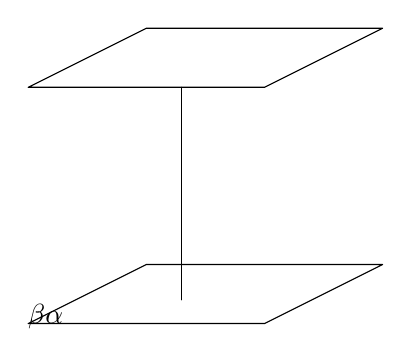
\begin{tikzpicture}[scale=1.5, font=\footnotesize, line join=round, line cap=round,>=stealth]
		\coordinate  (A) at (0,0); 
		\coordinate  (A') at (0,2);
		\coordinate (B) at (2,0);
		\coordinate  (B') at (2,2);
		\coordinate (C) at (3,0.5);
		\coordinate  (C') at (3,2.5);
		\coordinate (D) at (1,0.5);
		\coordinate  (D') at (1,2.5);
		\coordinate (M) at (1.3,2.2);
		\coordinate (H) at (1.3,.2);
		\coordinate (E) at (1.3,2.0);
		\draw (A) -- (B) --(C) -- (D)--(A)  (A') -- (B') -- (C')--(D')--(A');
		\draw (E) -- (H);
		\tkzDrawSegments[dashed](M,E)
		\tkzLabelPoints[left](M,H)
		\tkzDrawPoints[fill=black](M,H)
		\tkzMarkAngles[size=0.7](B,A,D)
		\tkzLabelAngle[pos=.4](D,A,B){$\beta$}
		\tkzMarkAngles[size=0.7](B',A',D')
		\tkzLabelAngle[pos=.4](D',A',B'){$\alpha$}
	\end{tikzpicture}
}
\subsubsection{Đường thẳng vuông góc chung và khoảng cách giữa hai đường thẳng chéo nhau}
\begin{itemize}
	\item [\iconMT] Đường vuông góc chung: Đường thẳng $\Delta$ cắt hai đường thẳng chéo nhau $a,b$ và cùng vuông góc với mỗi đường thẳng ấy được gọi là đường vuông góc chung của $a$ và $b$.
	\immini{
		\item [\iconMT] Khoảng cách giữa hai đường chéo nhau:
		\begin{itemize}
			\item [$\bullet$] Nếu đường thẳng vuông góc chung $\Delta$ cắt hai đường chéo nhau $a,b$ lần lượt tại $M,N$ thì độ dài đoạn $MN$ gọi là khoảng cách giữa hai đường thẳng chéo nhau $a$ và $b$.
			\item [$\bullet$] Kí hiệu $\mathrm{d}\left(a,b\right)$. Theo hình bên thì $\mathrm{d}\left(a,b\right)=MN.$
		\end{itemize}
	}{\hspace{1cm}
		\begin{tikzpicture}[scale=1, font=\footnotesize, line join=round, line cap=round,>=stealth]
			\tkzDefPoints{0/-1/A,0/1.5/B, 0/-2/C, 3/0/D,0/0/M, 1.5/-1/N}
			\tkzDrawSegments(A,B C,D M,N)
			\tkzMarkRightAngles(B,M,N M,N,D)
			\tkzLabelSegment[pos=0.8,above left](A,B){$a$}
			\tkzLabelSegment[pos=0.7,above](C,D){$b$}
			\tkzLabelPoints[below right](N)
			\tkzLabelPoints[above left](M)
			\tkzDrawPoints[fill=black](M,N)
	\end{tikzpicture}}
\end{itemize}

\begin{dang}{Khoảng cách từ một điểm đến một mặt phẳng}
	\begin{itemize}
		\item [] \indamm{Dựng khoảng cách từ $M$ đến $(\alpha)$, ta chú ý hai trường hợp đặc biệt sau:}
		\begin{itemize}
			\immini{\item [\iconMT] \indam{Trường hợp 1: } Nếu $M $ là hình chiếu vuông góc của một điểm $S \in (\alpha)$ xuống $(\beta)$. Khi đó khoảng cách từ $M$ đến $(\alpha)$ được dựng như sau:
				\begin{itemize}
					\item [$\bullet$] Bước 1. Dựng $MK$ vuông góc với giao tuyến $c$ tại $K$;
					\item [$\bullet$] Bước 2. Dựng $SK$.
					\item [$\bullet$] Bước 3. Dựng $MH \perp SK$ tại $H$. Suy ra
					$$\mathrm{d}(M,(\alpha))=MH.$$
			\end{itemize}}{\vspace{1cm}
				\begin{tikzpicture}[scale=1, line join=round, line cap=round]
					\tkzDefPoints{0/0/A,5/0/B, 6/2/C,1/2/D,2/2/E,2/1/M,2/4/S}
					\coordinate (K) at ($(C)!0.65!(B)$);
					\coordinate (H) at ($(S)!0.4!(K)$);
					\tkzDrawPolygon(S,B,C)
					\tkzDrawSegments(A,B A,D D,E S,M S,K M,B)
					\tkzDrawSegments[dashed](E,C M,K M,H M,C)
					\tkzMarkAngles[size=0.7cm,arc=l](B,A,D)
					\tkzLabelAngles[pos=0.4,rotate=30](B,A,D){\footnotesize $\beta$}
					\tkzMarkAngles[size=0.9cm,arc=l](B,S,C)
					\tkzLabelAngles[pos=1,rotate=30](B,S,C){\footnotesize $\alpha$}
					\tkzMarkRightAngle[size=0.2](M,K,B)
					\tkzMarkRightAngle[size=0.2](M,H,K)
					\tkzDrawPoints[size=5,fill=black](S,M,K,H)
					\tkzLabelPoints[below,font=\footnotesize](M)
					\tkzLabelPoints[left,font=\footnotesize](S)
					\tkzLabelPoints[below right,font=\footnotesize](K)
					\tkzLabelPoints[right,font=\footnotesize](H)
					\tkzLabelSegment[pos=0.7,right](B,C){$c$}
			\end{tikzpicture}}
			\immini{\item [\iconMT] \indam{Trường hợp 2:} Nếu $M\in (\beta)$ mà $(\alpha) \perp (\beta)$ thì khoảng cách từ $M$ đến $(\alpha)$ được dựng như sau: 
				\begin{itemize}
					\item [$\bullet$] Kẻ $MH$ vuông góc với giao tuyến $c$ tại $H$
					\item [$\bullet$] Suy ra $\mathrm{d}(M,(\alpha))=MH$.
			\end{itemize}}{
				\begin{tikzpicture}[scale=1, line join=round, line cap=round]
					\tkzDefPoints{0/0/A,4/0/B, 6/2/C,2/2/D,3/1/M}
					\coordinate (H) at ($(C)!0.65!(B)$);
					\coordinate (S) at ($(H)+(0,3)$);
					\tkzInterLL(M,S)(C,D)\tkzGetPoint{F}
					\tkzInterLL(M,H)(S,B)\tkzGetPoint{T}
					\tkzDrawPolygon(S,B,C)
					\tkzDrawSegments(A,B A,D M,B D,F S,M)
					\tkzDrawSegments[dashed](F,C F,C M,H M,C)
					\tkzMarkAngles[size=0.7cm,arc=l](B,A,D)
					\tkzLabelAngles[pos=0.4,rotate=30](B,A,D){\footnotesize $\beta$}
					\tkzMarkAngles[size=0.6cm,arc=l](B,S,C)
					\tkzLabelAngles[pos=0.4,rotate=30](B,S,C){\footnotesize $\alpha$}
					\tkzMarkRightAngle[size=0.2](M,H,B)
					\tkzDrawPoints[size=5,fill=black](S,M,H)
					\tkzLabelPoints[left,font=\footnotesize](M)
					\tkzLabelPoints[above,font=\footnotesize](S)
					\tkzLabelPoints[below right,font=\footnotesize](H)
					\tkzLabelSegment[pos=0.7,right](B,C){$c$}
			\end{tikzpicture}}
		\end{itemize}
		\begin{tcolorbox}[colframe=red,colback=yellow!3!white,boxrule=0.2mm]
			\begin{luuy}
				\immini{	\indamm{Trường hợp tổng quát, ta làm như sau: }
					\begin{itemize}
						\item [$\bullet$] Dựng mặt phẳng $(\beta)$ chứa điểm $M$ và $(\beta) \perp (\alpha)$
						\item [$\bullet$] Xác định giao tuyến $d$ của $(\beta)$ và $(\alpha)$.
						\item [$\bullet$] Kẻ $MH \perp d$ tại $H$ thì $MH \perp (\alpha)$. Suy ra $\mathrm{d}(M,(\alpha))=MH$.
				\end{itemize}}{
					\begin{tikzpicture}[line width=0.6pt,scale=1.2]
						\coordinate (A) at (0,0);
						\coordinate (B) at (1,1);
						\coordinate (C) at (4.3,1);
						\coordinate (D) at ($(A)+(C)-(B)$);
						\coordinate (A1) at ($(A)+(1.2,0)$);
						\coordinate (g) at (1.2,1);
						\coordinate (B1) at ($(B)+(1.8,0)$);
						\coordinate (C1) at ($(B)+(1.8,1.4)$);
						\coordinate (D1) at ($(A1)+(C1)-(B1)$);
						\coordinate (M) at (3.2,0.5);
						\coordinate (H) at ($(A1)!0.5!(B1)$);
						\clip (-0.1,-0.2) rectangle (4.4,2.4);
						\draw (g)--(B)--(A)--(A1)--(B1)--(C1)--(D1)--(A1)--(D)--(C)--(B1) (M)--(H);
						\draw[dashed] (g)--(B1);
						\node at (0.32, 0.12) {$\beta$};
						\draw (0.33,0.33)..controls(0.5,0.3)and(0.5,0.1)..(0.4,0);
						\draw (1.2,1.1)..controls(1.3,1.1)and(1.55,1.1)..(1.45,1.55);
						\node at (1.35, 1.3) {$\alpha$};
						\draw[fill=black] (M) circle(1pt);
						\node at ($(M)+(0.3,0)$) {$M$};
						\draw[fill=black] (H) circle(0.6pt);
						\node at ($(H)+(-0.15,0.15)$) {$H$};
						\node at ($(A1)+(0.2,0.35)$) {$d$};
						\tkzMarkRightAngle[size=0.17](B1,H,M)
				\end{tikzpicture}}
			\end{luuy}
		\end{tcolorbox}
	\end{itemize}
\end{dang}

\begin{dang}{Khoảng cách giữa đường và mặt phẳng song song. Khoảng cách giữa hai mặt song song}
	\begin{itemize}
		\item [\iconCH] \indamm{Cho đường thẳng $d$ song song với mặt phẳng $(\alpha)$:} Để tính khoảng cách giữa $d$ và $(\alpha)$ ta thực hiện
		\begin{itemize}
			\item Chọn điểm $A$ trên $d$ sao cho khoảng cách từ $A$ tới $(\alpha)$ được xác định dễ nhất.
			\item Kết luận $\mathrm{d}(d; (\alpha))=\mathrm{d}(A, (\alpha))$.
		\end{itemize}
		\item [\iconCH] \indamm{Cho hai mặt phẳng song song $(\alpha)$, $(\beta)$:} Để tính khoảng cách giữa hai mặt phẳng ta thực hiện các bước
		\begin{itemize}
			\item Chọn điểm $A$ trên $(\alpha)$ sao cho khoảng cách từ $A$ tới $(\beta)$ được xác định dễ nhất.
			\item Kết luận $\mathrm{d}((\beta); (\alpha))=\mathrm{d}(A, (\beta))$.
		\end{itemize}
	\end{itemize}
\end{dang}

\begin{dang}{Đoạn vuông góc chung. Khoảng cách giữa hai đường thẳng chéo nhau}
	\indamm{Dựng đoạn vuông góc chung:}
	\begin{itemize}
		\item [\iconMT] \indam{Trường hợp 1:}
		\immini{		
			Giả sử $a$ và $b$ là hai đường thẳng chéo nhau và $a \perp b$.
			\begin{itemize}
				\item[$\bullet$] Ta dựng mặt phẳng $(\alpha)$ chứa $a$ và vuông góc với $b$ tại $B$.
				\item[$\bullet$] Trong $(\alpha)$ dựng $BA \perp a$ tại $A$, ta được độ dài đoạn $AB$ là khoảng cách giữa hai đường thẳng chéo nhau $a$ và $b$.
			\end{itemize}
		}{
			\begin{tikzpicture}[scale=1, font=\footnotesize, line join=round, line cap=round,>=stealth]
				\tkzDefPoints{0/0/M,5/0/N,1.5/2.5/Q,6.5/2.5/P,2.5/-0.5/R,2.5/3.5/S,2.5/1.7/B,1.8/0.4/E,6/2.2/F}
				\tkzDefPointBy[homothety = center F ratio 0.4](E) \tkzGetPoint{A}
				\tkzInterLL(M,N)(R,S) \tkzGetPoint{I}
				\tkzDrawSegments(M,N N,P P,Q Q,M R,I B,S E,F A,B)
				\tkzDrawSegments[dashed](I,B)
				\tkzMarkAngles[size=1](N,M,Q)
				\tkzLabelAngles[color=black,pos=.6](Q,M,N){$\alpha$}
				\tkzLabelSegment[pos=0.9,right](R,S){$b$}
				\tkzLabelSegment[pos=0.9](E,F){$a$}
				\tkzMarkRightAngles[size=.3](B,A,F S,B,A)
				\tkzDrawPoints[fill=black](A,B)
				\tkzLabelPoints(A)
				\tkzLabelPoints[left](B)
			\end{tikzpicture}
		}
		\item [\iconMT] \indam{Trường hợp 2:}
		\immini{
			Giả sử $a$ và $b$ là hai đường thẳng chéo nhau nhưng không vuông góc với nhau.
			\begin{itemize}
				\item [$\bullet$] Ta dựng mặt phẳng $(\alpha)$ chứa $a$ và song song với $b$.
				\item [$\bullet$] Lấy một điểm $M$ tùy ý trên $b$ và dựng $MM'$ vuông góc với $(\alpha)$ tại $M'$.
				\item [$\bullet$] Từ $M'$ dựng $b'$ song song với $b$ cắt $a$ tại $A$.
			\end{itemize}
		}{
			\begin{tikzpicture}[scale=1, font=\footnotesize, line join=round, line cap=round,>=stealth]
				\tkzDefPoints{0/0/O,5/0/N,1.5/2.5/Q,6.5/2.5/P,1.6/3.5/R,5.5/3.5/S,1.6/1.8/E,4.7/3.5/M,4.7/1.8/M',2/2.3/G,4.8/0.2/H}
				\tkzDefPointBy[translation = from R to S](E) \tkzGetPoint{F}
				\tkzInterLL(G,H)(E,F) \tkzGetPoint{A}
				\tkzDefPointBy[translation = from M' to M](A) \tkzGetPoint{B}
				\tkzInterLL(P,Q)(A,B) \tkzGetPoint{J}
				\tkzInterLL(P,Q)(M,M') \tkzGetPoint{K}
				\tkzDrawSegments(O,N N,P P,K J,Q Q,O A,B M,M' R,S E,F G,H)
				\tkzDrawSegments[dashed](J,K)
				\tkzMarkAngles[size=1](N,O,Q)
				\tkzLabelAngles[color=black,pos=.6](Q,O,N){\normalsize $\alpha$}
				\tkzLabelSegment[pos=0.1,above](R,S){\normalsize $b$}
				\tkzLabelSegment[pos=0.9,above](G,H){\normalsize $a$}
				\tkzMarkRightAngles[size=.3](B,A,H A,B,M)
				\tkzDrawPoints[fill=black](A,B,M,M')
				\tkzLabelPoints[above](B,M)
				\tkzLabelPoints[below](A,M')
			\end{tikzpicture}
		}
		\begin{itemize}
			\item [$\bullet$] Từ $A$ dựng $AB$ song song với $MM'$ cắt $b$ tại $B$, độ dài đoạn $AB$ là khoảng cách giữa hai đường thẳng chéo nhau $a$ và $b$.
		\end{itemize}
	\end{itemize}
	\begin{luuy}
		\indam{Nhận xét:}
		\begin{itemize}
			\item Khoảng cách giữa hai đường thẳng chéo nhau bằng khoảng cách giữa một trong hai đường thẳng đó và mặt phẳng song song với nó chứa đường thẳng còn lại.
			\item Khoảng cách giữa hai đường thẳng chéo nhau bằng khoảng cách giữa hai mặt phẳng song song lần lượt chứa hai đường thẳng đó.
		\end{itemize}
	\end{luuy}
\end{dang}